\section{Regular Expressions}
Regular expressions are a way of matching multiple patterns with a single string, effectively providing a template. The basic symbols that can be used in a regular expression are :
\begin{description}
    \item [a,b,c$\dots$ :] Any single alphanumeric character
    \item [$\varepsilon$ :] An empty character
    \item [$|$ :] OR . e.g. $a|bs|cr$ represents the strings a, bs and cr
    \item [() :] Parentheses . e.g $(a|bs)cr$ represents acr and bscr
    \item [* :] 0 or more .e.g a* represents $\varepsilon$,a,aa,aaa,aaaa,$\dots$
    \item [+ :] 1 or more .e.g ba+ represents ba,baa,baa,$\dots$ \\
    \quad \textbf{a+ can be written as aa*}
    \item [? :] 0 or 1. e.g ca?r represents cr and car \\
    \quad \textbf{a? can be written as (a$|\varepsilon$)}
\end{description}
$|$ and * refer to the single character/parentheses block before them. Since ? and + can be re-written using $|$ and *, for the purpose of the below algorithms they're unused.

\subsection{Non-Deterministic Finite Automata (NFA)}
An automaton with two differences:
\begin{enumerate}
    \item $\varepsilon$-transitions, so a transition that can occur without a symbol for free movement from one state to the other
    \item A state doesn't need to have a transition for every symbol in the language, and can have multiple transitions for a single symbol.
\end{enumerate}
Any regular expression can be converted to an NFA, and vice-versa.

\newpage
\subsection{Thomson's Construction}
\begin{figure}[H]
    \centering
    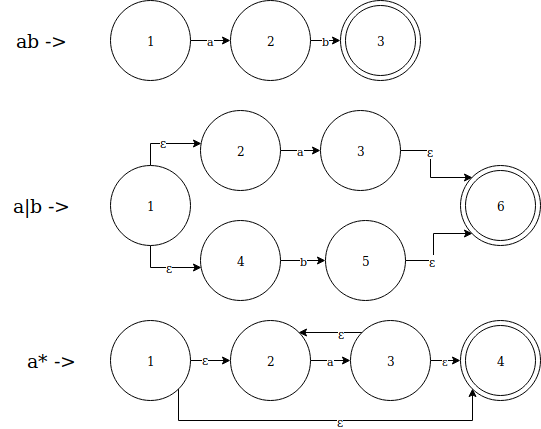
\includegraphics[width=\textwidth]{Regex/Regex1.png}
    \label{fig:Regex1}
\end{figure}
\begin{description}
    \item[Good] O($|s|$) construction, max. 2$|s|$ states, max. $|s|$ labelled transitions, \\max. 4$|s|\; \varepsilon$-transitions, max. 2 incoming/outgoing edges per state
    \item[Bad] Lots of $\varepsilon$-transitions, this causes a very large number of possible paths for checking a single text - O($|s|*$size($\sum$))
\end{description}

\newpage
\subsection{McNaughton and Yamada's Construction}
\begin{enumerate}
    \item Add a subscript to each character
    \item Make a table of potential successors for each character, and the possible Start/End Characters
    \item Construct the NFA
    \item Remove the subscripts
\end{enumerate}
\textbf{e.g.}
\begin{align}
    s &= ab(a|\varepsilon)a(b^*|ba) \nonumber \\
    s &= a_1b_2(a_3|\varepsilon)a_4(b^*_5|b_6a_7) \nonumber 
\end{align}

\begin{table}[H]
\centering
\begin{tabular}{|l|l|}
\hline
Character & Successor \\ \hline
START & $a_1$ \\ \hline
$a_1$ & $b_2$ \\ \hline
$b_2$ & $a_3, a_4$ \\ \hline
$a_3$ & $a_4$ \\ \hline
$a_4$ & END,$ b_5, b_6$ \\ \hline
$b_5$ & $END,b_5$ \\ \hline
$b_6$ & $a_7$ \\ \hline
$a_7$ & END \\ \hline
\end{tabular}
\label{tab:Regex2.23}
\end{table}
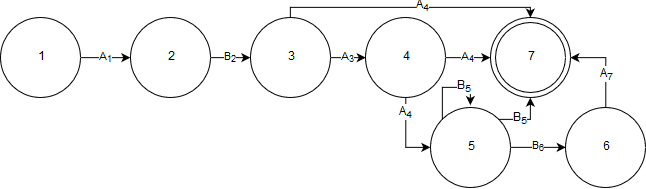
\includegraphics[width=\textwidth]{Regex/Regex24.png}
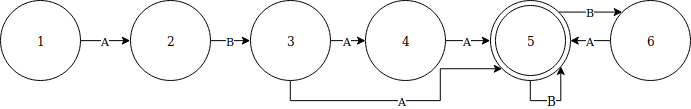
\includegraphics[width=\textwidth]{Regex/Regex25.png}
\begin{description}
    \item[Good] $|s|+1$ states , no $\varepsilon$-transitions
    \item[Bad] Making the table can be $O(|s| + |s|^2)$
\end{description}